\documentclass[tikz, border=2pt]{standalone}
\usetikzlibrary{shapes.geometric, arrows, positioning}
\usetikzlibrary{backgrounds}

\tikzset{
  double -latex/.style args={#1 colored by #2 and #3}{    
    -latex,line width=#1, #2,
    postaction={draw, -latex, #3, line width=(#1)/3, shorten <=(#1)/4, shorten >=4.5*(#1)/3},
  },
  box/.style  = {draw, rectangle, minimum width=5cm, minimum height=1.2cm, text centered, text width=5cm},
  myarrow/.style = {double -latex=4mm colored by blue and blue!40},
}

\begin{document}
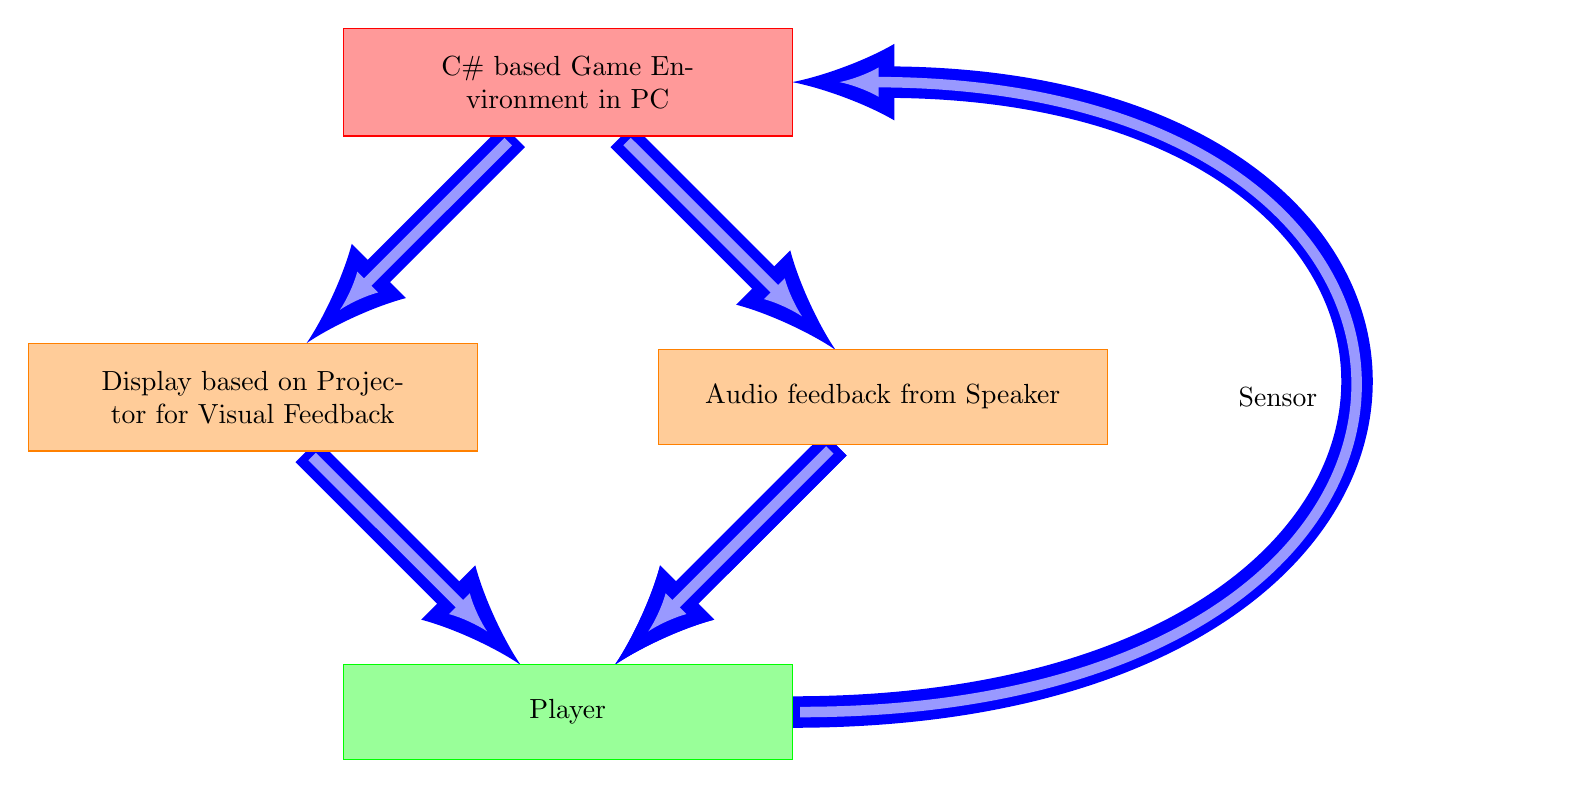
\begin{tikzpicture}[node distance=4cm, every node/.style={inner sep=10pt, outer sep=0pt, font=\normalsize, text=black}]
    \node (n00) [box, draw=red, fill=red!40] {C\# based Game Environment in PC};
    \node (n10) [box, draw=orange, fill=orange!40, below of=n00, xshift=-4cm] {Display based on Projector for Visual Feedback};
    \node (n11) [box, draw=orange, fill=orange!40, below of=n00, xshift=+4cm] {Audio feedback from Speaker};
    \node (n20) [box, draw=green, fill=green!40, below of=n10, xshift=+4cm] {Player};

    \begin{scope}[on background layer]
        \draw [myarrow] (n00) -- (n10);
        \draw [myarrow] (n00) -- (n11);
        \draw [myarrow] (n10) -- (n20);
        \draw [myarrow] (n11) -- (n20);
        \draw [myarrow] (n11) -- (n20);
        \draw [myarrow] (n20.east)  to [out=0, in=0, looseness=3] node[left]{Sensor} (n00.east);
    \end{scope}
\end{tikzpicture}
\end{document}
